\documentclass[twocolumn, a4paper]{article}
\usepackage[a4paper, left = 1.75cm, right = 1.75cm, top = 1.75cm, bottom = 1.75cm]{geometry}
\usepackage[style = numeric, sorting = none]{biblatex}
\usepackage{pgfplots}
\usepackage[T1]{fontenc}
\usepackage{graphicx}
\usepackage[UKenglish]{babel}
\usepackage[UKenglish]{isodate}

\graphicspath{{./images/}}
\addbibresource{refs.bib}

\cleanlookdateon

\renewcommand*{\bibfont}{\footnotesize}

\author{
  George Herbert\\
  \texttt{cj19328@bristol.ac.uk}
}

\title{\vspace{-2em}Parallelising d2q9-bgk.c with MPI}

\begin{document}

\maketitle

\begin{abstract}
  \texttt{d2q9-bgk.c} implements the Lattice Boltzmann method (LBM) to simulate a fluid density on a lattice.
  This report analyses the techniques I utilised to parallelise \texttt{d2q9-bgk.c} with MPI, and port \texttt{d2q9-bgk.c} to a GPU with OpenCL.
\end{abstract}

\section{Single Program, Multiple Data}

\subsection{Hypothesis}

I previously achieved a substantial performance improvement producing a multithreaded implementation of \texttt{d2q9-bgk.c} with OpenMP.
However, since OpenMP was built for shared-memory parallelism, my implementation could not utilise more than one node of BC4, which was a considerable restriction.

Single program, multiple data (SPMD) is a form of parallelism in which independent processes run the same program.
Message Passing Interface (MPI) is a specification for a library interface for passing messages between processes.
Therefore, I hypothessied that a parallel implementation of \texttt{d2q9-bgk.c} that ran on multiple processes across multiple nodes---with MPI being used for interprocess communication---would provide an even more substantial performance improvement.

I opted to use the implementation of my program prior to enforcing single instruction, multiple data (SIMD) vectorization as a starting point.
I was uncertain the changes I previously implemented to enforce SIMD vectorization would provide a performance benefit to my MPI implementation.

\subsection{Load Balancing}

I had to explicitly assign different sections of the grid to different processes.
It was crucial for the distribution to be adequately balanced to minimise the amount of time processes' spent blocked.

Since the \texttt{cells} grid was stored in row-major order, I split the grid horizontally between processes to take advantage of memory locality.
I created a procedure \texttt{allocate\_rows} to balance the load; the procedure assigned each process at least $\lfloor\frac{y}{n}\rfloor$ consecutive rows, with the first $y - \lfloor\frac{y}{n}\rfloor n$ processes each assigned an additional consecutive row, where $y$ was the number of rows and $n$ the number of processes.
Additionally, since updating the value of a given cell required the values of all adjacent cells, each process contained two additional rows reserved for cells in the top and bottom rows of the preceding and succeeding ranks, respectively.
Figure \ref{fig:rows} displays an example allocation for a grid with five rows, split between two processes; the rows allocated to a specific process are highlighted in green, with additional rows required to correctly updated the edge rows highlighted in red.

\begin{figure}[htbp]
  \centering
  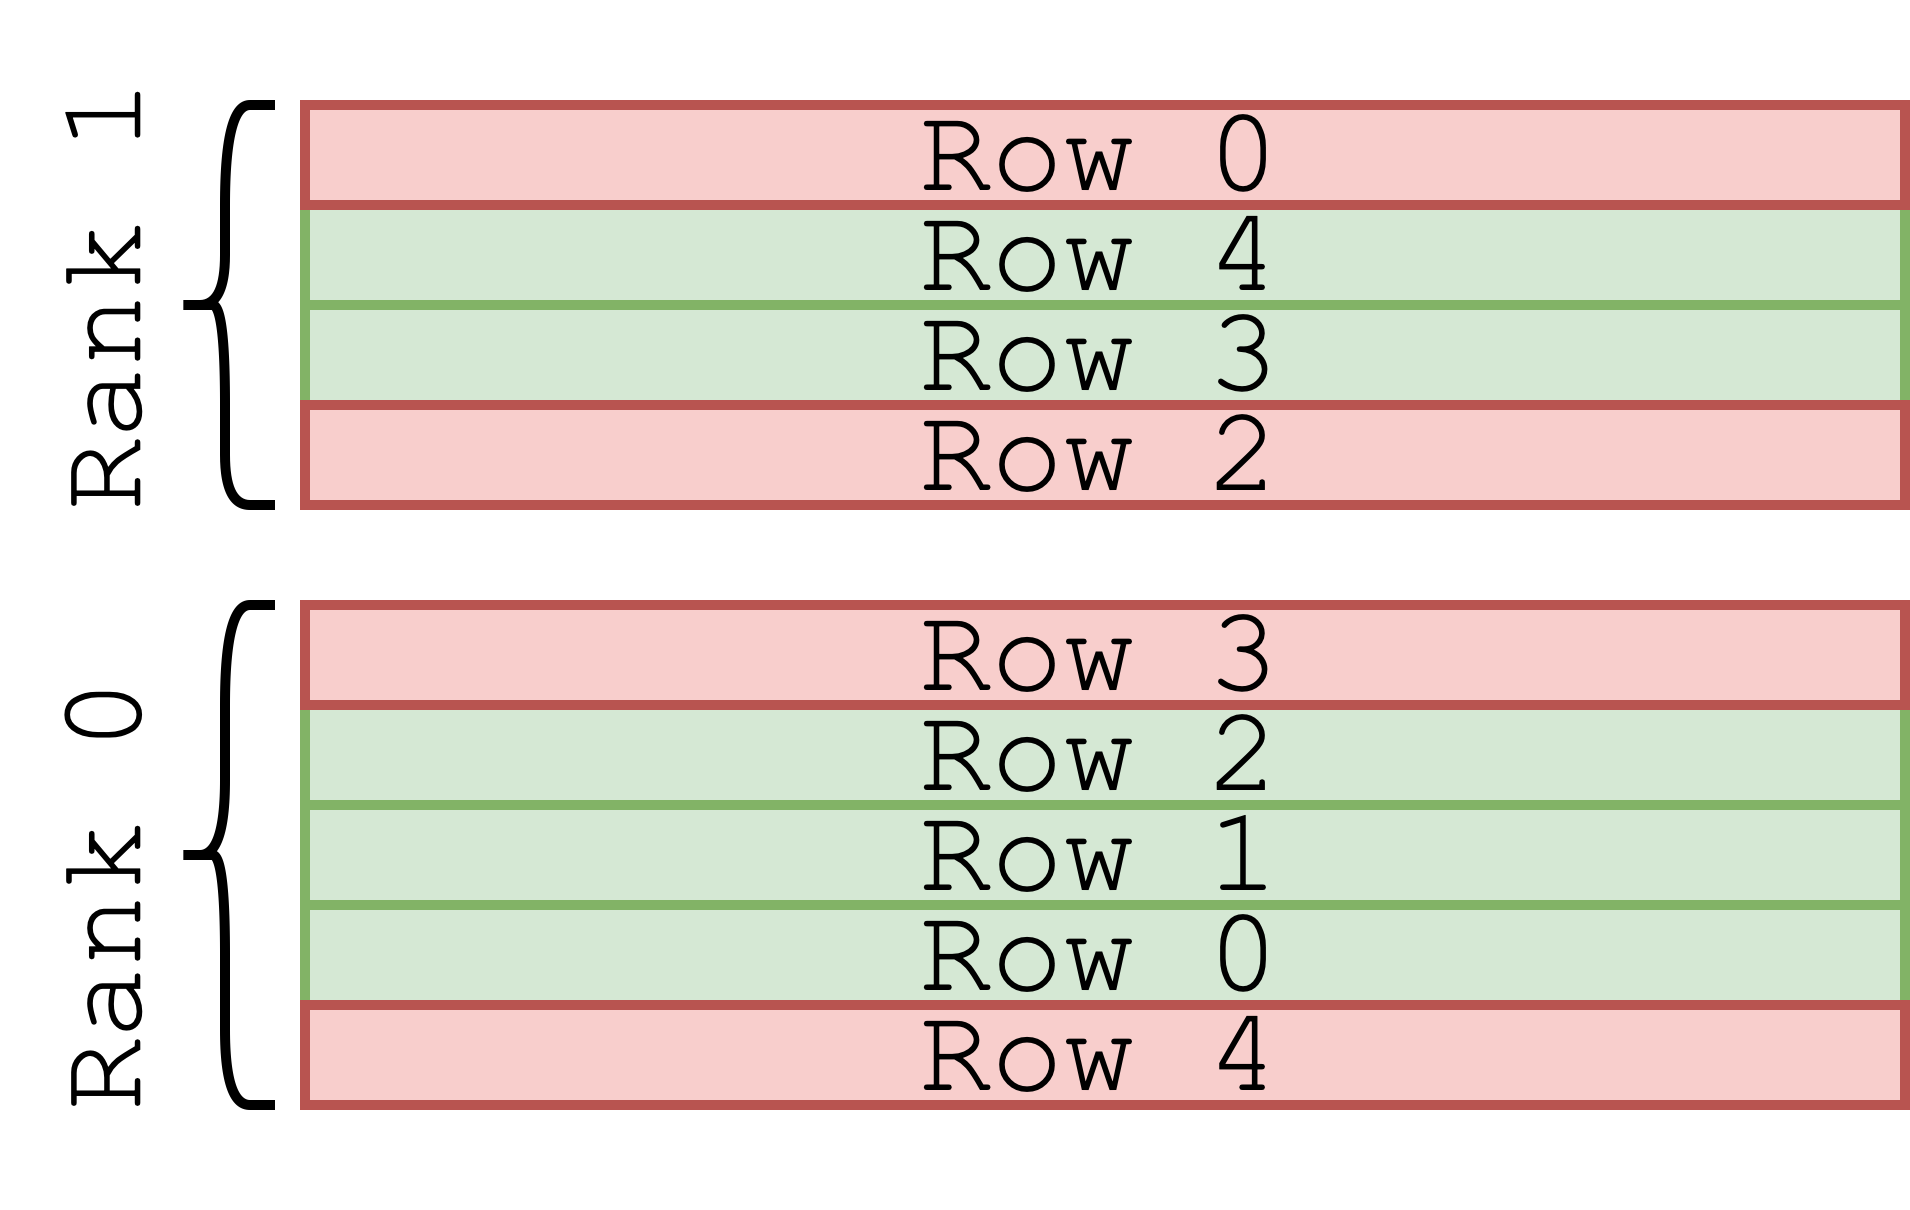
\includegraphics[width=.75\linewidth]{rows.png}
  \caption{Row allocation example with five rows and two processes}\label{fig:rows}
\end{figure}

I decided against splitting on a sub-row level to avoid unnecessarily increasing the complexity of my program and incurring an additional computational overhead.

\subsection{Halo Exchange}

Since processes are assigned their own virtual memory region, I had to explicitly send the contents of edge rows to neighbouring ranks at the conclusion of each timestep.
To do so, I created a \texttt{halo\_exchange} procedure.
The procedure copied the bottom-most row allocated to each process into the \texttt{send\_row\_buffer} array.
I used the \texttt{MPI\_Sendrecv} procedure to send this buffer to the \texttt{receive\_row\_buffer} of the preceding rank.
The values in the \texttt{receive\_row\_buffer} were then copied into the top additional row.
The same process was then repeated for the top-most row, which was sent to the succeeding rank.

\subsection{Collating}

I created a \texttt{collate} procedure to be executed once all iterations of the \texttt{timestep} procedure have been completed.
The procedure had two purposes.
The first purpose was to transfer the the final state of the cells allocated to each process to the master process (i.e. rank zero).
The second purpose was to transfer the partial average velocity values to the master process, and use these values to calculate the correct average velocity at each timestep.

I used the \texttt{MPI\_Send} procedure to transfer the final state of the cells allocated to each process to the master process.
The master process received these values by executing the \texttt{MPI\_Recv} procedure once for each timestep.

I used the \texttt{MPI\_Reduce} procedure to sum the partial average velocity values held by each process.
Once the arrays had been summed, I multiplied each element by \texttt{params.num\_non\_obstacles\_r} in the master process to calculate the correct average velocity at each timestep.

\subsection{Results}

\begin{table}[htbp]
  \begin{center}
  \caption{Execution times with the 52 process MPI implementation and speedup over both the prior and 28 thread OpenMP implementation}\label{tab:mpi}
  \begin{tabular}[t]{l | l  l  l} 
      \hline\hline
      &&\multicolumn{2}{c}{Speedup}\\
      \cline{3-4}
      Grid Size&Time (s)&Prior&OpenMP\\
      \hline
      $128 \times 128$&\texttt{}&\texttt{}&\texttt{}\\
      $128 \times 256$&\texttt{}&\texttt{}&\texttt{}\\
      $256 \times 256$&\texttt{}&\texttt{}&\texttt{}\\
      $1024 \times 1024$&\texttt{}&\texttt{}&\texttt{}\\
      \hline
    \end{tabular}
  \end{center}
\end{table}

Each time was an average of five runs on a BlueCrystal Phase 4 (BC4) compute node---a Lenovo nx360 M5, which contained two 14-core 2.4 GHz Intel E5-2680 v4 (Broadwell) CPUs and 128 GiB of RAM \cite{bcp4}.

\section{Optimisations}

\subsection{Average Velocities Reduction}

\begin{table}[htbp]
  \begin{center}
  \caption{Collate times with the reduction and speedup over the prior implementation}\label{tab:reduction}
  \begin{tabular}[t]{l | l l} 
      \hline\hline
      Grid Size&Time (s)&Speedup\\
      \hline
      $128 \times 128$&\texttt{0.0016}&\texttt{4.54}\\
      $128 \times 256$&\texttt{0.0029}&\texttt{2.93}\\
      $256 \times 256$&\texttt{0.0049}&\texttt{2.83}\\
      $1024 \times 1024$&\texttt{0.0420}&\texttt{1.08}\\
      \hline
    \end{tabular}
  \end{center}
\end{table}

\subsection{Vectorization}

I hypothesised that SIMD vectorization of the inner loop would drastically improve the performance of my MPI implementation, as it did with my serial optimised implementation previously.
Therefore, I made the same changes as I did with my serial optimised implementation, including converting the cells' data from an array of structures (AoS) to a structure of arrays (SoA) format.
However, the SoA format meant that the \texttt{halo\_exchange} procedure had to be altered since the \texttt{MPI\_Sendrecv} procedure required the address of a single buffer as input.

I experimented with two separate approaches to send a row in the \texttt{halo\_exchange} procedure.
The first approach involved nine separate calls to the \texttt{MPI\_Sendrecv procedure}, one for each of the nine arrays in the SoA.
The second approach involved copying the cells' values in each of the nine arrays into a large buffer, followed by a single call to the \texttt{MPI\_Sendrecv} procedure.

Table \ref{tab:vectorization_1} and Table \ref{tab:vectorization_2} display the results for the first and second approach, respectively.
The second approach was significantly faster, since the overhead introduced by nine separate calls to the \texttt{MPI\_Sendrecv} procedure was larger than the overhead introduced by copying the values within the nine arrays into a single buffer.

\begin{table}[htbp]
  \begin{center}
  \caption{Execution times with the first vectorization approach and speedup over the prior implementation}\label{tab:vectorization_1}
  \begin{tabular}[t]{l | l l} 
      \hline\hline
      Grid Size&Time (s)&Speedup\\
      \hline
      $128 \times 128$&\texttt{}&\texttt{}\\
      $128 \times 256$&\texttt{}&\texttt{}\\
      $256 \times 256$&\texttt{}&\texttt{}\\
      $1024 \times 1024$&\texttt{}&\texttt{}\\
      \hline
    \end{tabular}
  \end{center}
\end{table}

\begin{table}[htbp]
  \begin{center}
  \caption{Execution times with the second vectorization approach and speedup over the prior implementation}\label{tab:vectorization_2}
  \begin{tabular}[t]{l | l l} 
      \hline\hline
      Grid Size&Time (s)&Speedup\\
      \hline
      $128 \times 128$&\texttt{}&\texttt{}\\
      $128 \times 256$&\texttt{}&\texttt{}\\
      $256 \times 256$&\texttt{}&\texttt{}\\
      $1024 \times 1024$&\texttt{}&\texttt{}\\
      \hline
    \end{tabular}
  \end{center}
\end{table}

\section{Experiments}

\subsection{Hybrid MPI and OpenMP}

I also experimented with a hybrid MPI and OpenMP implementation.
In this implementation, each of the four compute nodes contained a single process.

\begin{table}[htbp]
  \begin{center}
  \caption{Execution times with the hybrid implementation and speedup over the prior implementation}\label{tab:hybrid}
  \begin{tabular}[t]{l | l l} 
      \hline\hline
      Grid Size&Time (s)&Speedup\\
      \hline
      $128 \times 128$&\texttt{}&\texttt{}\\
      $128 \times 256$&\texttt{}&\texttt{}\\
      $256 \times 256$&\texttt{}&\texttt{}\\
      $1024 \times 1024$&\texttt{}&\texttt{}\\
      \hline
    \end{tabular}
  \end{center}
\end{table}

\subsection{OpenMP vs MPI}

\begin{figure}[htpb]
  \centering
  \resizebox{\columnwidth}{!}{
    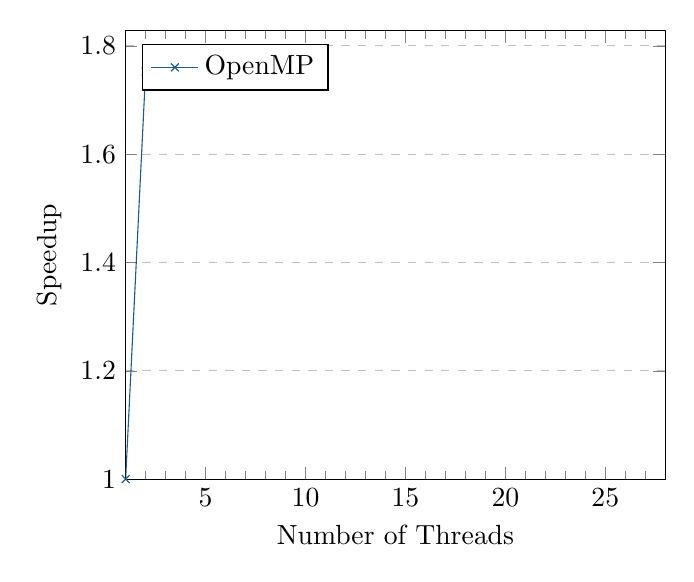
\begin{tikzpicture}
      \begin{axis}[
        xlabel={Number of Threads},
        ylabel={Speedup},
        xmin = 1, xmax = 28,
        ymin = 1,
        % xtick={0, 5, 10, 15, 20, 25},
        % ytick={0,20,40,60,80,100,120},
        legend pos=north west,
        ymajorgrids=true,
        grid style=dashed,
        minor xtick = {1, 2, 3, 4, 5, 6, 7, 8, 9, 10, 11, 12, 13, 14, 15, 16, 17, 18, 19, 20, 21, 22, 23, 24, 25, 26, 27, 28}
      ]
      \addlegendentry{OpenMP}
      \addplot[color = {rgb:red,31;green,119;blue,180}, mark = x]coordinates{
        (1, 1.0)
        (2, 1.7525169788462858)
      };
      \addlegendentry{MPI}
      \addplot[color = {rgb:red,255;green,127;blue,14}, mark = x]coordinates{
      };
      \end{axis}
    \end{tikzpicture}
  }
  \caption{Speedup curves for my OpenMP and MPI implementation on the $1024\times1024$ grid}\label{fig:scaling_openmp_mpi}
\end{figure}

\subsection{Scaling}

I ran my final MPI implementation from 1--112 processes to analyse how my program scaled.
My program ran on as few nodes as possible, such that each process was assigned to a single core. 
I then calculated the subsequent processes' speedup over a single process implementation.
Figure \ref{fig:scaling} displays the result speedup curves.

\begin{figure}[htpb]
  \centering
  \resizebox{\columnwidth}{!}{
    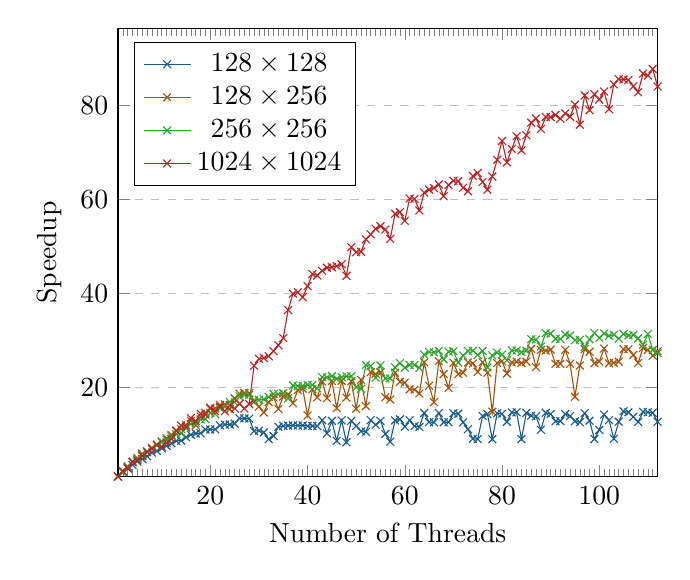
\begin{tikzpicture}
      \begin{axis}[
        xlabel={Number of Threads},
        ylabel={Speedup},
        xmin = 1, xmax = 112,
        ymin = 1,
        % xtick={0, 5, 10, 15, 20, 25},
        % ytick={0,20,40,60,80,100,120},
        legend pos=north west,
        ymajorgrids=true,
        grid style=dashed,
        minor xtick = {1, 2, 3, 4, 5, 6, 7, 8, 9, 10, 11, 12, 13, 14, 15, 16, 17, 18, 19, 20, 21, 22, 23, 24, 25, 26, 27, 28, 29, 30, 31, 32, 33, 34, 35, 36, 37, 38, 39, 40, 41, 42, 43, 44, 45, 46, 47, 48, 49, 50, 51, 52, 53, 54, 55, 56, 57, 58, 59, 60, 61, 62, 63, 64, 65, 66, 67, 68, 69, 70, 71, 72, 73, 74, 75, 76, 77, 78, 79, 80, 81, 82, 83, 84, 85, 86, 87, 88, 89, 90, 91, 92, 93, 94, 95, 96, 97, 98, 99, 100, 101, 102, 103, 104, 105, 106, 107, 108, 109, 110, 111, 112}
      ]
      \addlegendentry{$128\times128$}
      \addplot[color = {rgb:red,31;green,119;blue,180}, mark = x]coordinates{
        (1, 1.0)
        (2, 1.9355629603956905)
        (3, 2.6952632289306426)
        (4, 3.489894687089785)
        (5, 4.200247140003777)
        (6, 4.724752446853035)
        (7, 5.308227888248851)
        (8, 6.078118911191303)
        (9, 6.443290980821596)
        (10, 7.014442733994245)
        (11, 7.535972554765394)
        (12, 8.055979511566001)
        (13, 8.593785454403191)
        (14, 8.637121428079936)
        (15, 9.366410830401875)
        (16, 9.895596516254974)
        (17, 10.161810937870444)
        (18, 10.22575107795616)
        (19, 11.002128645305085)
        (20, 11.020850231204689)
        (21, 11.037671024945826)
        (22, 11.8937812320222)
        (23, 12.052108670604802)
        (24, 12.064105703242813)
        (25, 12.255796653353853)
        (26, 13.37712380488399)
        (27, 13.376648617926609)
        (28, 13.326469532509947)
        (29, 10.67595348893722)
        (30, 10.774420862243385)
        (31, 10.381199553401766)
        (32, 8.956079014963102)
        (33, 9.637157319206578)
        (34, 11.577096051649171)
        (35, 11.765260646690336)
        (36, 11.834349837591278)
        (37, 11.90229332321905)
        (38, 11.857026869592401)
        (39, 11.876927305332023)
        (40, 11.752933229595579)
        (41, 11.765391928443266)
        (42, 11.73140924364138)
        (43, 12.995538311361777)
        (44, 10.16951447695839)
        (45, 12.84307124133966)
        (46, 8.587290366297024)
        (47, 12.95087637413253)
        (48, 8.291072591222623)
        (49, 12.867929870465879)
        (50, 11.77472042739376)
        (51, 10.615354876902042)
        (52, 10.498832019978135)
        (53, 12.98804661131778)
        (54, 12.036781745660278)
        (55, 12.853999702542772)
        (56, 10.076487587825595)
        (57, 8.402067376191706)
        (58, 12.943022964632403)
        (59, 13.1729633294354)
        (60, 11.609192263735876)
        (61, 12.968525611223034)
        (62, 11.741363758855613)
        (63, 11.5588711198032)
        (64, 14.519955382348487)
        (65, 12.589437437016729)
        (66, 12.53093647273583)
        (67, 14.521155196870996)
        (68, 12.53460106420919)
        (69, 12.551850405698831)
        (70, 14.461525379095438)
        (71, 14.368468819583933)
        (72, 12.53856600255434)
        (73, 11.070281461820809)
        (74, 9.025304168742393)
        (75, 8.955105382597942)
        (76, 13.873334245594828)
        (77, 14.304803199600594)
        (78, 8.950620281253025)
        (79, 14.477609317116439)
        (80, 14.32003455075865)
        (81, 12.633907517110485)
        (82, 14.650284142223951)
        (83, 14.663731312147974)
        (84, 8.976299202141243)
        (85, 14.53612954635065)
        (86, 13.93501371832758)
        (87, 13.832638025220005)
        (88, 10.94707094030582)
        (89, 14.5659698622416)
        (90, 14.295028714906262)
        (91, 12.736707576343255)
        (92, 12.792088865595154)
        (93, 14.296734408304722)
        (94, 13.864103865502903)
        (95, 12.771666743380967)
        (96, 12.557201961713712)
        (97, 14.466922418335088)
        (98, 12.881134873765816)
        (99, 8.964043358129649)
        (100, 10.910144075758767)
        (101, 14.196598941713455)
        (102, 13.010643995014869)
        (103, 9.048275980434223)
        (104, 12.66784727395055)
        (105, 14.87553258127684)
        (106, 14.658512510670006)
        (107, 13.68644615612271)
        (108, 12.620086416354475)
        (109, 14.749267009847808)
        (110, 14.693361204013376)
        (111, 14.565446704111881)
        (112, 12.65209941251008)
      };
      \addlegendentry{$128\times256$}
      \addplot[color = {rgb:red,255;green,127;blue,14}, mark = x]coordinates{
        (1, 1.0)
        (2, 2.1211824026559607)
        (3, 3.1482880693011857)
        (4, 4.190159900979048)
        (5, 4.939707332890799)
        (6, 5.854973417955859)
        (7, 6.398502763405941)
        (8, 7.117747211718579)
        (9, 7.779658093948965)
        (10, 8.489259833330294)
        (11, 9.151410859442448)
        (12, 9.875491502125529)
        (13, 10.812639529536366)
        (14, 11.1282971889931)
        (15, 12.0031837116075)
        (16, 12.880059007692468)
        (17, 11.90755465976407)
        (18, 13.77983987838145)
        (19, 14.573251526060416)
        (20, 15.4350434661521)
        (21, 15.493026611626794)
        (22, 16.25132197927561)
        (23, 16.36325714012558)
        (24, 15.31665971365891)
        (25, 17.6264414121068)
        (26, 18.64634380797662)
        (27, 18.803325885392177)
        (28, 18.734678404651408)
        (29, 16.83276807395762)
        (30, 15.87878651446253)
        (31, 14.631419950971148)
        (32, 16.820312601617204)
        (33, 17.857595708737954)
        (34, 15.373064755803584)
        (35, 18.034637287032517)
        (36, 18.487202702895893)
        (37, 16.61355999463276)
        (38, 19.421396210357685)
        (39, 19.68573859388584)
        (40, 13.986354410391558)
        (41, 19.57413103841477)
        (42, 17.832232215361515)
        (43, 21.20957428003375)
        (44, 17.694589256963543)
        (45, 21.336330687961635)
        (46, 15.560533134390617)
        (47, 21.36864920243236)
        (48, 17.80530614680176)
        (49, 21.292183486641346)
        (50, 15.413579928087566)
        (51, 21.56060036272223)
        (52, 15.988047321671424)
        (53, 23.215048959083408)
        (54, 22.79956628460271)
        (55, 23.175478351948353)
        (56, 17.87973472046407)
        (57, 17.401793323704347)
        (58, 23.083089549249014)
        (59, 21.152562611319105)
        (60, 20.979985434775557)
        (61, 19.551310889106524)
        (62, 19.485158311345646)
        (63, 18.665722038856437)
        (64, 25.286766479165173)
        (65, 20.3215230452524)
        (66, 16.841317547230968)
        (67, 25.557409160080724)
        (68, 22.804703756970596)
        (69, 19.87120198053611)
        (70, 25.185316705509642)
        (71, 22.79202063285041)
        (72, 23.092615998174587)
        (73, 25.2757283957052)
        (74, 25.0547613153221)
        (75, 23.262796117591563)
        (76, 25.318671780335578)
        (77, 23.09573211993007)
        (78, 14.794758398714578)
        (79, 25.15548615088671)
        (80, 25.552246965296025)
        (81, 22.895323583914642)
        (82, 25.29022816166884)
        (83, 25.414151141157667)
        (84, 25.16288275978371)
        (85, 25.45517236854192)
        (86, 28.172422473911872)
        (87, 24.278163226140215)
        (88, 27.945338987120504)
        (89, 27.78376358922697)
        (90, 28.006668046317774)
        (91, 24.987843759460162)
        (92, 24.98306994835336)
        (93, 27.944735104505565)
        (94, 24.99637679603101)
        (95, 17.983502271392812)
        (96, 24.61250190326346)
        (97, 28.10466416333627)
        (98, 27.56229041547468)
        (99, 25.123773607714206)
        (100, 25.447436029185077)
        (101, 28.22934322290837)
        (102, 25.10063708279057)
        (103, 25.1935488758913)
        (104, 25.4372023490791)
        (105, 28.095505129752564)
        (106, 28.098693152874315)
        (107, 26.870086484340007)
        (108, 25.151300292603654)
        (109, 28.39387211909333)
        (110, 27.956683409118753)
        (111, 26.7112283632992)
        (112, 27.664690599737106)
      };
      \addlegendentry{$256\times256$}
      \addplot[color = {rgb:red,44;green,160;blue,44}, mark = x]coordinates{
        (1, 1.0)
        (2, 1.9260934439078088)
        (3, 3.0639634815233845)
        (4, 4.085545063947559)
        (5, 4.777349060288223)
        (6, 5.558264790927939)
        (7, 6.348195798982507)
        (8, 6.879282922522227)
        (9, 7.658287872646965)
        (10, 8.263681026247555)
        (11, 8.819975046843068)
        (12, 9.559154759245137)
        (13, 9.989263709355136)
        (14, 10.238621877231742)
        (15, 11.315387099365147)
        (16, 12.190383044726568)
        (17, 12.381318700042957)
        (18, 13.144720606492987)
        (19, 13.209890340155061)
        (20, 14.58776164295752)
        (21, 14.30145253410522)
        (22, 15.551472352395859)
        (23, 15.841170618870756)
        (24, 16.901285308440563)
        (25, 16.803820300937346)
        (26, 18.039504458635346)
        (27, 18.420945797795902)
        (28, 18.37618326761103)
        (29, 17.25110582425766)
        (30, 17.29254153461277)
        (31, 17.444468732192203)
        (32, 17.947810916730077)
        (33, 18.551290325903757)
        (34, 18.504776690874404)
        (35, 18.722993357677364)
        (36, 17.63637099123006)
        (37, 20.37466352624495)
        (38, 20.22726113977795)
        (39, 20.309952557831636)
        (40, 20.49049944690594)
        (41, 20.475406432323567)
        (42, 19.757555780497647)
        (43, 22.192249701825055)
        (44, 22.086712754203123)
        (45, 22.362524923831472)
        (46, 21.806456130523074)
        (47, 22.13309699670076)
        (48, 22.325326954246616)
        (49, 22.352097968329314)
        (50, 20.023385904160044)
        (51, 19.66858309688602)
        (52, 24.722205376754847)
        (53, 24.479638715076764)
        (54, 22.01232774715682)
        (55, 24.63357297661218)
        (56, 21.847854227349885)
        (57, 21.874566071935014)
        (58, 24.21001704461762)
        (59, 25.130217412276366)
        (60, 24.15963046526658)
        (61, 24.757656633956202)
        (62, 24.750170753292416)
        (63, 24.091727334277955)
        (64, 26.949790484618187)
        (65, 27.496817709560812)
        (66, 27.424501598051215)
        (67, 27.74358617114127)
        (68, 25.91707381172878)
        (69, 27.566250097337058)
        (70, 27.68102649168171)
        (71, 25.26217193742185)
        (72, 26.74591742837863)
        (73, 27.704096559612317)
        (74, 27.78331897835484)
        (75, 26.8637568248063)
        (76, 27.730230994907696)
        (77, 24.22783241866554)
        (78, 26.7713992635353)
        (79, 27.389536471576275)
        (80, 26.957929362880886)
        (81, 25.749921355006606)
        (82, 27.832813326335692)
        (83, 27.815037822214105)
        (84, 27.489828020134226)
        (85, 27.79883351007423)
        (86, 30.23334481782003)
        (87, 30.128047822443612)
        (88, 28.679403653112843)
        (89, 31.50579857207405)
        (90, 31.413300670077092)
        (91, 30.314798617855892)
        (92, 30.249441476444876)
        (93, 31.20632435486909)
        (94, 30.979495395551726)
        (95, 30.02089211899462)
        (96, 30.08799621090498)
        (97, 28.55879643547644)
        (98, 30.20353733202267)
        (99, 31.53016630405491)
        (100, 30.5211422457308)
        (101, 31.420664301818547)
        (102, 30.92991843095905)
        (103, 31.172433361205336)
        (104, 30.336558258496467)
        (105, 31.31729458385978)
        (106, 31.03137031900762)
        (107, 31.127336320416525)
        (108, 30.402761445464755)
        (109, 29.027628344037428)
        (110, 31.347965908119033)
        (111, 27.923595160195326)
        (112, 27.25334229964955)
      };
      \addlegendentry{$1024\times1024$}
      \addplot[color = {rgb:red,214;green,39;blue,40}, mark = x]coordinates{
        (1, 1.0)
        (2, 2.175065592912396)
        (3, 2.8043033777244397)
        (4, 4.049123378845032)
        (5, 4.464167860970939)
        (6, 5.364090309825796)
        (7, 6.165070196050448)
        (8, 6.869352759321628)
        (9, 7.754483711755721)
        (10, 7.393992763845299)
        (11, 8.21945041573844)
        (12, 9.027950565438944)
        (13, 10.688317225061487)
        (14, 11.864630140696315)
        (15, 11.617515309270185)
        (16, 13.452397210362253)
        (17, 12.799788703157422)
        (18, 14.36504915814569)
        (19, 14.18585904184895)
        (20, 15.627328763798452)
        (21, 14.89686026821259)
        (22, 15.889264997445022)
        (23, 14.889064582966338)
        (24, 16.207887686949775)
        (25, 15.462722295207566)
        (26, 16.492684128209376)
        (27, 15.47709325955812)
        (28, 16.42924409485685)
        (29, 24.56871693810117)
        (30, 26.040386007762798)
        (31, 26.22366435089637)
        (32, 26.588595625724643)
        (33, 27.69137971965659)
        (34, 28.921792405334546)
        (35, 30.453346119716127)
        (36, 36.42685999522134)
        (37, 39.91337338653539)
        (38, 40.2193770595146)
        (39, 39.15394779198545)
        (40, 41.514925701278536)
        (41, 44.09725875018143)
        (42, 43.78449929147865)
        (43, 44.79883014556155)
        (44, 45.41963627169753)
        (45, 45.55355044910432)
        (46, 45.7775718987104)
        (47, 46.17858806643465)
        (48, 43.71833000960987)
        (49, 49.81813677470648)
        (50, 48.74121497908254)
        (51, 48.82097464603227)
        (52, 51.467797181941734)
        (53, 52.54164390528638)
        (54, 53.73814706329768)
        (55, 54.25701823287112)
        (56, 53.5639858945203)
        (57, 51.564478372996916)
        (58, 56.90630594884924)
        (59, 57.24737877488094)
        (60, 55.40287831689169)
        (61, 60.172337160151926)
        (62, 60.06545844820975)
        (63, 57.60195571917357)
        (64, 61.40242480519957)
        (65, 62.044676725408145)
        (66, 62.38437688337686)
        (67, 63.149902369818925)
        (68, 60.64323784067146)
        (69, 63.063667697148084)
        (70, 63.94536187303647)
        (71, 63.83941964827168)
        (72, 62.43715831437613)
        (73, 61.69744451132279)
        (74, 64.94087437535914)
        (75, 65.57515298825429)
        (76, 63.67767680455072)
        (77, 62.03944796307024)
        (78, 64.84614723609315)
        (79, 68.38578901467969)
        (80, 72.40237225618469)
        (81, 67.85454464590445)
        (82, 70.71028058099046)
        (83, 73.40860273164466)
        (84, 70.39941565207157)
        (85, 73.6224039779562)
        (86, 76.28867690987647)
        (87, 77.1747933744947)
        (88, 74.95431769174382)
        (89, 77.50534090143563)
        (90, 77.47428261488723)
        (91, 77.92167062981707)
        (92, 77.11543301941525)
        (93, 78.27544880348194)
        (94, 77.53028540496351)
        (95, 80.14633028483333)
        (96, 75.86966091470653)
        (97, 82.08444144503459)
        (98, 78.947471321217)
        (99, 82.32319951828144)
        (100, 81.22041635885635)
        (101, 82.9174143484004)
        (102, 79.15964280437144)
        (103, 84.4334159050141)
        (104, 85.57448174866816)
        (105, 85.49143450908768)
        (106, 85.3793510367548)
        (107, 84.03903495519286)
        (108, 82.7721252897915)
        (109, 86.74681171822564)
        (110, 86.33592220588343)
        (111, 87.71682878165659)
        (112, 83.9960192709098)
      };
      \end{axis}
    \end{tikzpicture}
  }
  \caption{Speedup curves for my MPI implementation}\label{fig:scaling}
\end{figure}

In general, my implementation initially scaled well for the smallest three grid sizes, but the speedup acquired from each subsequent process declined (i.e. a sublinear plateau), which occurred due to several reasons.
Perfect linear scaling was theoretically impossible because the program contained serial sections.

A different pattern emerged in the largest grid size.

Notably, the amount of speedup provided by each next core was approximately inversely proportional to the test case size.
In other words, larger grid sizes benefitted more from a multiprocess implementation than smaller grid sizes.
Firstly, this was because the larger grids benefitted more from being split sufficiently small to fit into the faster cache levels.
Secondly, the larger grid sizes were more evenly divided by the number of processes.

\section{Comparison to Serial}

\section{GPU Programming}

GPUs typically have 3--5x the memory bandwidth, and 5--10x the peak FLOP/s that CPUs have.
This is true for BC4, in which the Nvidia Pascal P100 has 4.8x the memory bandwidth and 9.8x the performance that the Intel E5-2680 v4 has.
OpenCL is a framework for heterogeneous computing that can be used for GPU programming.

I sought to identify whether I could produce an implementation of LBM in OpenCL to run on a single GPU in BCP4 that would be faster than my MPI implementation on one node.

\subsection{Original Code}

\begin{table}[htbp]
  \begin{center}
  \caption{Execution times with the OpenCL implementation and speedup over the serial implementation}\label{tab:OpenCL_1}
  \begin{tabular}[t]{l | l l} 
      \hline\hline
      Grid Size&Time (s)&Speedup\\
      \hline
      $128 \times 128$&\texttt{}&\texttt{}\\
      $128 \times 256$&\texttt{}&\texttt{}\\
      $256 \times 256$&\texttt{}&\texttt{}\\
      $1024 \times 1024$&\texttt{}&\texttt{}\\
      \hline
    \end{tabular}
  \end{center}
\end{table}

\subsection{Optimisations}

\begin{table}[htbp]
  \begin{center}
  \caption{Execution times with the OpenCL implementation and speedup over the prior implementation}\label{tab:OpenCL_2}
  \begin{tabular}[t]{l | l l} 
      \hline\hline
      Grid Size&Time (s)&Speedup\\
      \hline
      $128 \times 128$&\texttt{}&\texttt{}\\
      $128 \times 256$&\texttt{}&\texttt{}\\
      $256 \times 256$&\texttt{}&\texttt{}\\
      $1024 \times 1024$&\texttt{}&\texttt{}\\
      \hline
    \end{tabular}
  \end{center}
\end{table}

\section{Conclusion}

\printbibliography

\end{document}